\section{Background} \label{background}

\onehalfspacing

\subsection{Prior Art} \label{sec:prior-art}

Finding and receiving emergency medical attention during emergencies with calls to 911 is common in most communities. Receiving emergency medical attention via a mobile app, however, is not. Only one app, PulsePoint, was found that currently provides a similar service.

PulsePoint \cite{pulsepoint} is a suite of mobile apps released in October of 2016 that can be used by 911 operators to direct CPR certified users to heart attacks incidents and defibrillators during emergencies. When someone reports a heart attack or heart failure to a 911-center integrated with PulsePoint's technology, the emergency operator notifies all qualified users nearby of the location of the person in need. A registered responder can then navigate to the emergency and perform CPR or administer a defibrillator. To date, the app has helped save numerous lives and has been adopted in various locations across the country. A version of PulsePoint's model of incorporating emergency call centers into the network is discussed in Section \ref{sec:alt-user-ex}. Other apps and websites such as AED Locations \cite{aedlocations} and HeartSafe \cite{heartsafe} allow users to manually search and find AEDs in their communities, but do not integrate with 911 services as PulsePoint does.

No product or service was found that provides a mobile app for finding or receiving autoinjectors in emergencies. 

\subsection{Population Considerations} \label{sec:population}

In this application, autoinjectors are the only devices crowdsourced. They are designed to be carried at all times by those with prescriptions, unlike defibrillators which are bulky and typically stored in cabinets. A crowdsourcing network is useful only if certain population and active-user requirements hold. Specifically, for the network to be used within a particular geographic area, the population density of autoinjector carriers must be high enough to make sharing autoinjectors logistically possible within a reasonable amount of time. Based on this necessity, the following probabilistic measure is considered:

\begin{adjustwidth}{2.5em}{0pt}
    In the event that Person $X$ is looking for an autoinjector in Area $A$, what is the probability that there exists some Autoinjector Carrier $Y$ such that the distance between $X$ and $Y$ makes it possible for $Y$ to walk to $X$ faster than an ambulance could travel to $X$?
\end{adjustwidth}

This asks whether this network is useful based on the population densities of people who carry autoinjectors. This probability will be used to show that the network effect of sharing autoinjectors is, in fact, possible. I address this question in the following two sections.

\subsubsection{Autoinjectors Nearby} \label{autoinjectors-nearby}

Let $R$ be the event that Person $X$ is having an allergic reaction and needs an autoinjector in area $A$. Let the random variable $N$ be the number of autoinjector carriers nearby Person $X$ in Area $A$, where nearby is defined to be walking distance within 8 minutes and will be further derived and defined below. To determine the usefulness of a peer-to-peer network of autoinjectors, I find the probability that there are at least $k$ autoinjector carriers nearby Person $X$, given that Person $X$ has a reaction in Area $A$. Thus, I am looking for $P(N \geq k|R)$. For purposes of simplicity, I assume that Person $X$ having a reaction does not increase the probability that someone with an autoinjector is nearby, and thus assume $N$ is independent of $R$. Thus, I determine the probability that there are at least $k$ people carrying autoinjectors in area $A$ at any given time, or
\begin{align*}
    P(N \geq k)
\end{align*}
By taking the complement,
\begin{align*}
    P(N \geq k) &= 1 - P(N < k) \\
    &= 1 - \sum_{j=0}^{k-1}P(N=j).
\end{align*}
Therefore, in order to evaluate $P(N \geq k)$, the probability mass function (PMF) of $N$, $P(N=k)$, needs to be determined. According to the U.S. Census Bureau, population varies drastically during normal working hours, so I account for this in the model by using different population statistics between 8:00 AM and 5:00 PM and 5:00 PM and 8:00 AM \cite{acs}. Additionally, Person $X$ might be more likely to be eating and, thus, more likely to have a reaction during working hours. However, eating behaviors are difficult to model and vary among different populations; therefore, I ignore eating behaviors in this model and assume independence. Let $W$ be the event that the current time is between 8:00 AM and 5:00 PM. Then $P(W) = 9/24$ and $P(W^c) = 15/24$. By the Law of Total Probability \cite{blitz},
\begin{align*}
    P(N=k) = P(N=k|W)P(W)+ P(N=k|W^c)P(W^c).
\end{align*}
Next, I need to clarify a few definitions. First, I define an autoinjector carrier near Person $X$ to be a person with an autoinjector who could, on average, walk to Person $X$ faster than an ambulance could drive to Person $X$. While there is no federally-mandated ambulance response time standards, many cities and municipalities choose to set an 8-minute response time as the gold standard \cite{ems}. The National Fire Protection Agency also recommends that Advanced Life Support teams should aim to respond to all calls within 8 minutes \cite{nfpa}. In actuality, average response times vary across regions, with some cities averaging below 8 minutes and some above \cite{nycems}\cite{bostonems}.  Therefore, for the purposes of analysis, I assume that the average response time of an ambulance to Person $X$ is 8 minutes. Now, the effective nearby Area $A$ around Person $X$ is anywhere within an 8-minute walk from Person $X$. The average walking speed of adults is 5 km/h \cite{walking}. I thus calculate $A$ as
\begin{align*}
    A &= \pi r^2 \\
    &= \pi\left(\left(5\text{ km/h}\right)\left(8\text{ min}\right)\left(1/60 \text{ h/min}\right)\right)^2 = 1.40 \text{ km}^2.
\end{align*}
Now, I determine the probability that a person within Area $A$ has an autoinjector. According to Food Allergy Research and Education, 12\% of people within the U.S. have food allergies, with children and adults accounting for 8\% and 4\% respectively \cite{food}; however, the subject of interest is people who are carrying autoinjectors, not necessarily those who have allergies. According to John Lee, M.D., Director of the Food Allergy Program at Boston Children's Hospital, more than 4.5 million autoinjector twin packs were prescribed in 2015 for children and adults combined \cite{johnlee}. Because food allergies are on the rise \cite{food}, I assume that the number of autoinjectors prescribed next year will at least remain the same despite recent rate increases \cite{wsjepi}. Let $m$ be the number of unexpired autoinjector twin packs prescribed to consumers. Most autoinjectors expire 1.5 years after the date of manufacture, so I assume that
\begin{align*}
    m = 1.5(4.5 \times 10^6) = 6.75 \times 10^6.
\end{align*}
The population of the U.S. is $u=$ 321,418,820 \cite{acs}. Let $T$ be the event that a given person in the U.S. has a prescription for an autoinjector twin pack.
\begin{align*}
    P(T) &= m/u \\
    &= \frac{6.75 \times 10^6}{321418820}\\
    &= 0.021
\end{align*}
While this is a simplistic model, it serves as a decent approximation.\footnote{More granular prescription data for autoninjectors prescribed was not found. Ideally, the analysis should use the number of users in a given city and number of prescriptions in that city. Instead, I perform the analysis with the naive definition.} In reality, infants should not be included in the total population. I could try and treat population of children and adults differently who might have different probabilities of having prescriptions, but parents of those children might be just as likely to carry an autoinjector as their children. Therefore, I assume this probability for purposes of analysis. I do account for the fact that a person with a prescription may not have the autoinjector on their person at all times. Let $P(C)$ be the probability that any given owner or user of an autoinjector is actually carrying it on their person. Then, assuming independence, the probability $p$ that any given person has an autoinjector on their person is 
\begin{align*}
    p = P(T)P(C)
\end{align*}
Let $\rho$ be the population density of Area $A$ around Person $X$. The number of people, $n$, in Area $A$ is modeled as
\begin{align*}
    n = \left\lfloor\rho A \right\rfloor.
\end{align*}
Each person in Area $A$ has an independent probability $p$ of having an autoinjector on their person. This is the story of the binomial distribution \cite{blitz}, as each person's having an autoinjector can be modeled as an independent Bernoulli trial with probability of success $p$. Thus, the number of pens during working and non-working hours both have the binomial distribution, so
\begin{align*}
    N|W,N|W^c \sim \text{Bin}(n,p).
\end{align*}
For any random variable $X \sim \text{Bin}(n,p)$, the PMF of $X$ is
\begin{align*}
    P(X=k) = \binom{n}{k}p^k(1-p)^{n-k}.
\end{align*}
Therefore, $P(N=k)$ is
\begin{align*}
    P(N=k) &= P(N=k|W)P(W) + P(N=k|W^c)P(W^c) \\
    &= \left(\binom{n_W}{k}p^k(1-p)^{n_W-k}\right)\left(9/24\right) + \left(\binom{n_{W^c}}{k}p^k(1-p)^{n_{W^c}-k}\right)\left(15/24\right),
\end{align*}
where $n_W$ and $n_{W^c}$ are the populations of Area $A$ during working hours and non-working hours respectively. Now, I can use this to determine $P(N\geq k)$---the probability that there are at least $k$ autoinjectors near Person $X$ in Area $A$---if the population density of Area $A$ is known, since $n=\left\lfloor \rho A \right\rfloor$. Using U.S. Census Bureau data for population densities \cite{acs}, Figure \ref{fig:nyandhouston} shows $P(N \geq k)$ for New York City and Houston, and each line represents a different value for $P(C)$. The population density of New York City is 10908 people/km$^2$ while Houston is 1480 people/km$^2$, and as expected the number of autoinjetors likely to be in any given area is much higher in New York City.

\begin{figure}[h]
\centering
\begin{subfigure}{.5\textwidth}
  \centering
  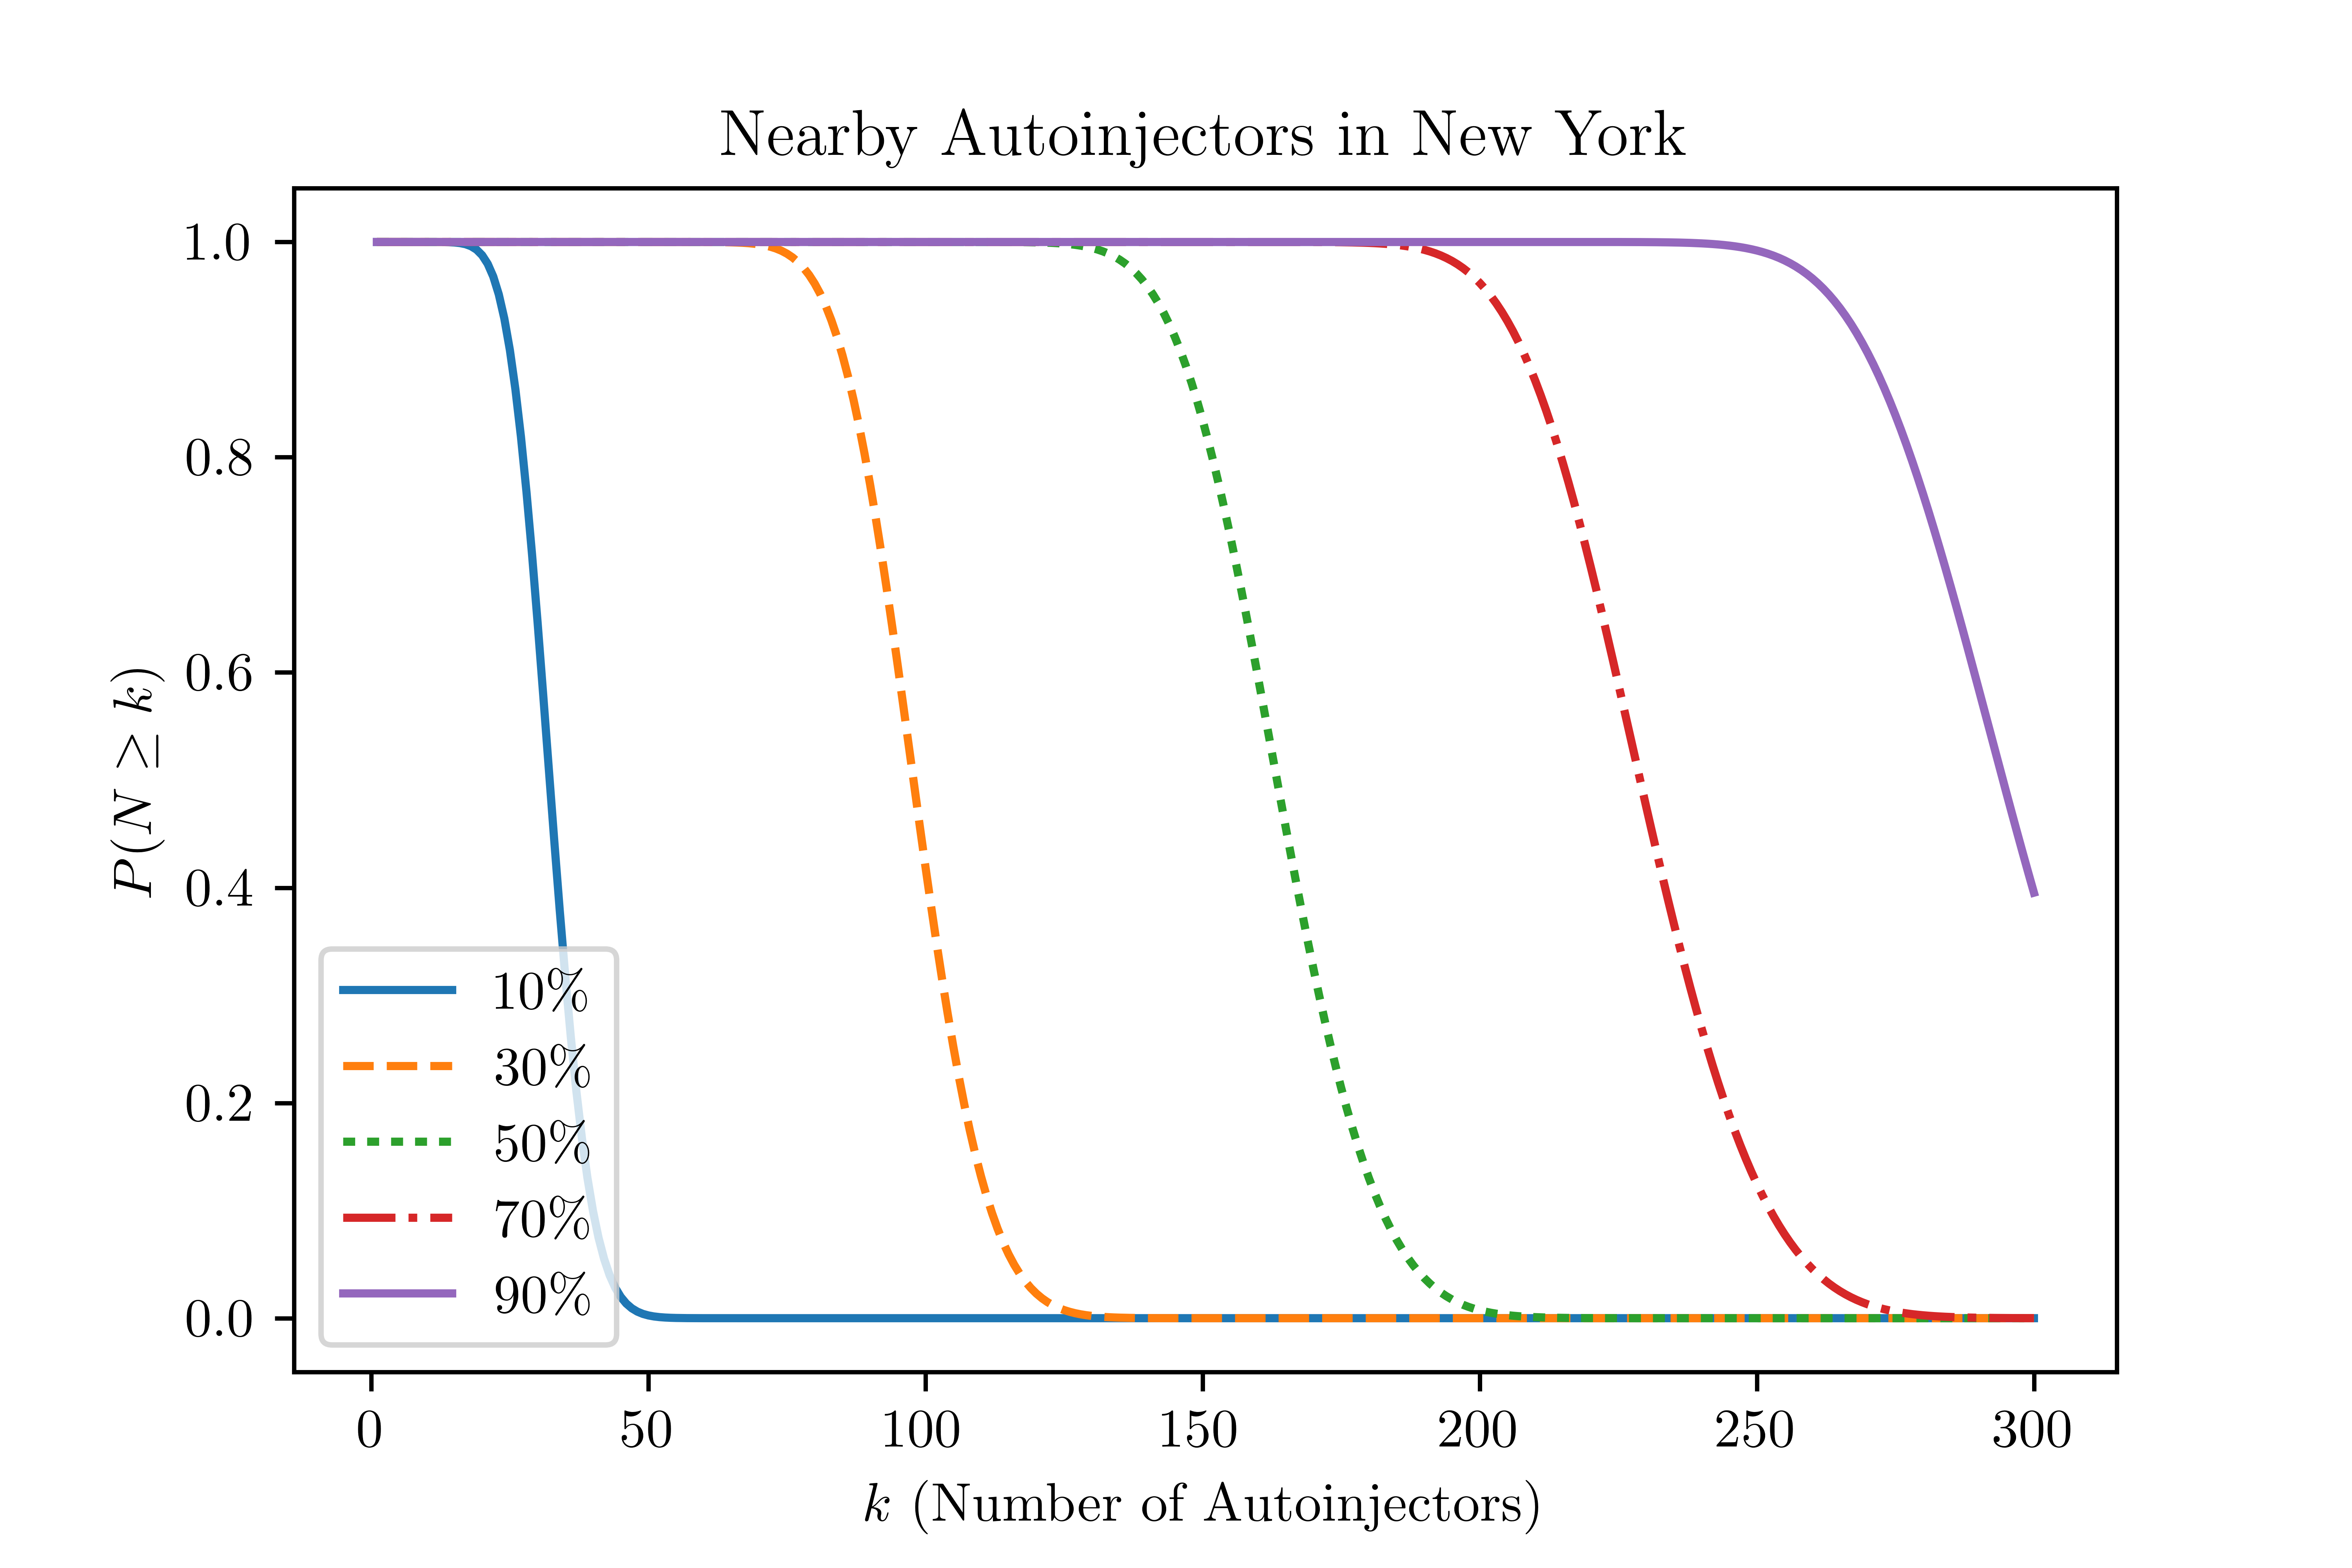
\includegraphics[width=\linewidth]{NewYork-cmfs}
%  \caption{A subfigure}
  \label{fig:newyorkcmf}
\end{subfigure}%
\begin{subfigure}{.5\textwidth}
  \centering
  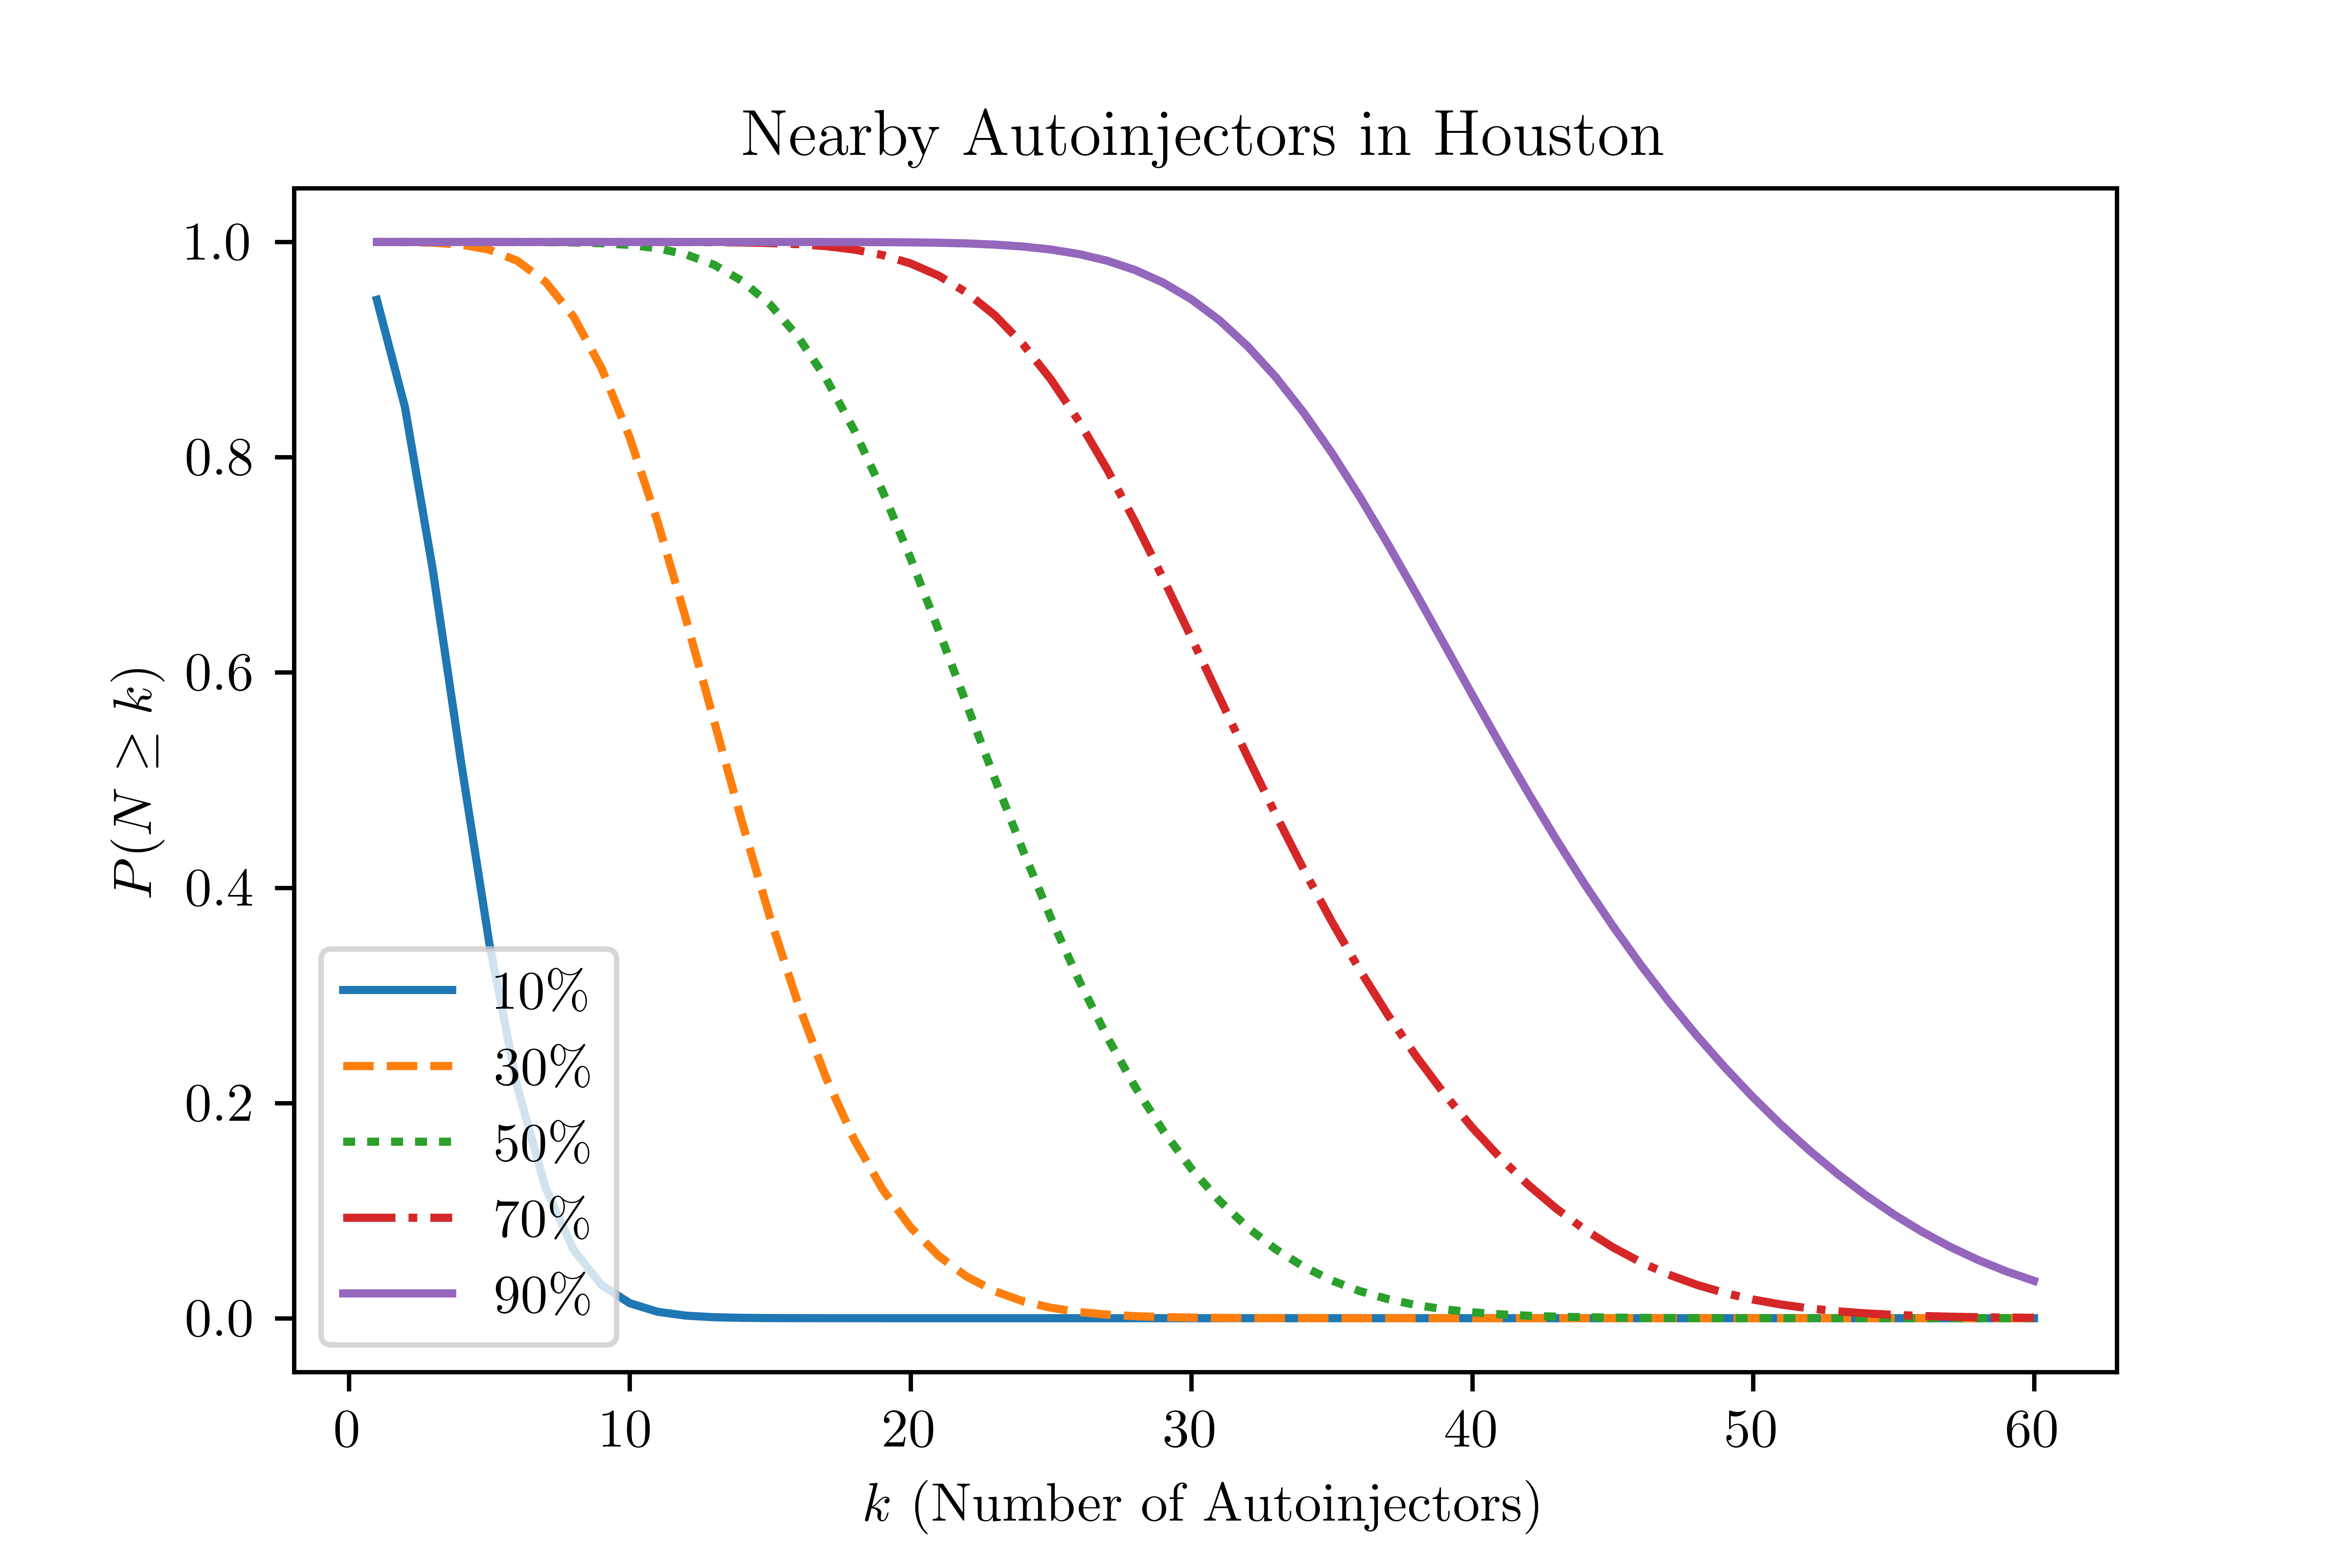
\includegraphics[width=\linewidth]{Houston-cmfs}
%  \caption{A subfigure}
  \label{fig:houstoncmf}
\end{subfigure}
\caption{$P(N\geq k)$ for New York City and Houston. Each line represents a different value for $P(C)$, the probability that a person with a prescription is carrying an autoinjector, ranging from 10\% to 90\%.}
\label{fig:nyandhouston}
\end{figure}

As can be seen, a higher population density corresponds to an increase in the expected number of autoinjectors nearby. As shown in Figure \ref{fig:nyandhouston}, even if 50\% of people with autoinjector prescriptions carry it on their person, there is only a 50\% chance there will be at least 25 autoinjectors nearby in Houston compared to New York's 160. New York and Houston are the first and fourth largest populated cities in the U.S. respectively \cite{acs}, yet there is a significant difference in likelihood due to their differing population densities. I next consider this effect more formally and determine the number of people living in different population densities in the U.S. and the resulting effect on $P(N \geq k)$.

\subsubsection{Population Densities}

As shown in Section \ref{autoinjectors-nearby} through the cities of New York and Houston, a higher population density corresponds to an increase in the expected number of autoinjectors nearby. Figure \ref{fig:denscomp} shows this effect of population density on $P(N\geq k)$ for two different values of $P(C)$. As expected, the probability of having an autoinjector nearby is proportional to population density. 

\begin{figure}[h]
\centering
\begin{subfigure}{.5\textwidth}
  \centering
  \includegraphics[width=\linewidth]{{{dencomp-pc-0.3}}}
%  \caption{A subfigure}
  \label{fig:den03}
\end{subfigure}%
\begin{subfigure}{.5\textwidth}
  \centering
  \includegraphics[width=\linewidth]{{{dencomp-pc-0.5}}}
%  \caption{A subfigure}
  \label{fig:den05}
\end{subfigure}
\caption{Comparing $P(N\geq k)$ for different population densities. As the population density increases, the chances of having more autoinjectors nearby increases. The graph on the left assumes $P(C) = 0.3$ while the right assumes $P(C) = 0.5$. The unit of population density, $\rho$, is people/km$^2$.}
\label{fig:denscomp}
\end{figure}

An important consideration that arrises from this analysis is determining how many people in the U.S. live in an area with a population density that allows a reasonable probability of having an autoinjector nearby. If the number is too low, then an implementation of this network might not be  practical. Figure \ref{fig:popbydensity} shows $uP(T)P(C)$---the number of people in the U.S. population who have prescriptions for autoinjectors and carry them on their person---living in different population densities. The y-axis shows the number who live in an area of at least the density of the value on the x-axis.

\begin{figure}[h]
\centering
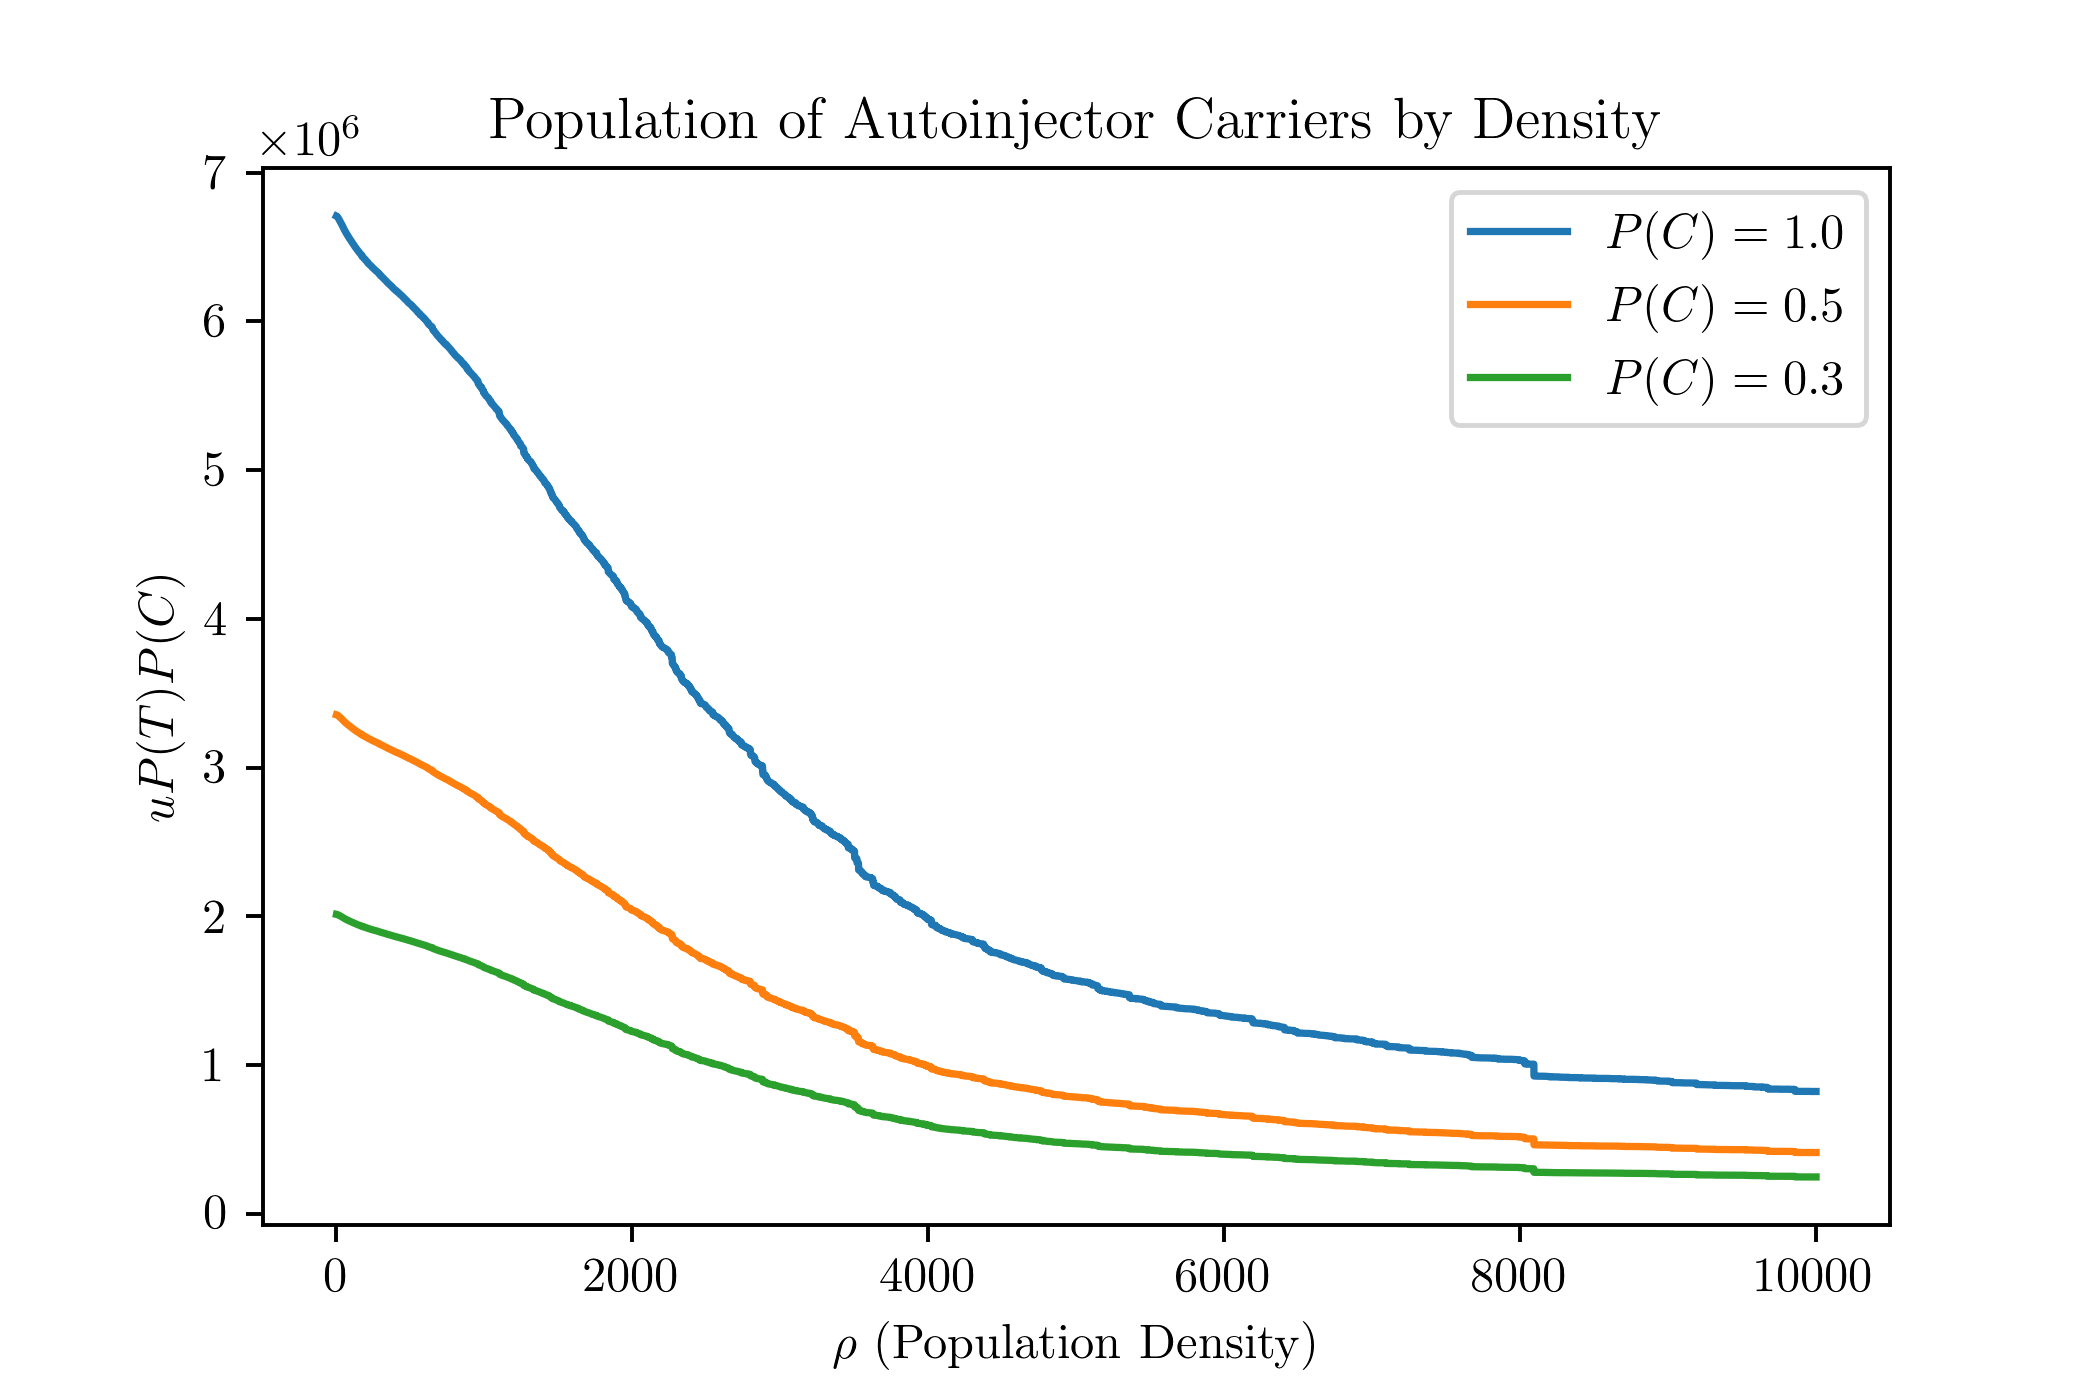
\includegraphics[width=0.5\textwidth]{popbydensity}
\caption{Population of autoinjector carriers who live in areas of differing population densities. The y-axis shows the number of autoinjector carriers who live in an area of at least the density of the value on the x-axis.}
\label{fig:popbydensity}
\end{figure}

The relationship between Figures \ref{fig:denscomp} and \ref{fig:popbydensity} combine to show how many autoinjector prescribers live in areas where $P(N \geq k) > 0.5$ for different values of $k$. These results are shown in Table \ref{tab:probsforks}. Recall that $P(C) = 1.0$ means that everyone with an autoinjector is carrying it on their person, and thus $uP(T)P(C)$ represents the total number of people with autoinjector prescriptions. Thus, for any value of $k$ in Table \ref{tab:probsforks}, $uP(T) : P(N\geq k) > 0.5$ indicates of the total number of people \textit{who might need} an autoinjector living in areas where $P(N \geq k) > 0.5$. As can be seen, over 6 million people who might need an autoinjector live an area where it is more likely than not that there are at least 10 autoinjectors within walking distance, even if only 30\% of prescribers are carrying their autoinjector.

\begin{table}[h]
\centering
\begin{tabular} {|c||c|c|}
    \hline
    & \multicolumn{2}{|c|}{$uP(T) : P(N\geq k) > 0.5$} \\\hline
    $k$ & $P(C) = 0.3$ & $P(C) = 0.5$ \\\hline\hline
    10 & $6.06 \times 10^{6}$ & $6.31 \times 10^{6}$ \\\hline
    20 & $4.89 \times 10^{6}$ & $5.09 \times 10^{6}$ \\\hline
    50 & $3.11 \times 10^{6}$ & $3.34 \times 10^{6}$ \\\hline
    90 & $9.89 \times 10^{5}$ & $1.50 \times 10^{6}$ \\\hline 
\end{tabular}
\caption{Population of autoinjector carriers living in areas where the probability of having at least $k$ autoinjectors nearby $P(N \geq k)$, is at least $1/2$ for different values of $k$ and $P(C)$.}
\label{tab:probsforks}
\end{table}

These results indicate that millions of people who might need an autoinjector in an emergency live in areas where a crowdsourcing app could, on average, supply one faster than an ambulance. Based on these results, I conclude that creating such a crowdsourcing network is indeed possible.